\documentclass{article}
\usepackage[utf8]{inputenc}
\usepackage{graphicx}% Include figure files
\usepackage{hyperref}  
\usepackage{color}
\usepackage{verbatim}
\usepackage{amsmath}
\usepackage{polski}
\usepackage[section]{placeins}
\usepackage{caption}
\usepackage{subcaption}

\title{MPiS - Zadanie domowe 2}
\author{Michał Łukomski}
\date{\today}

\begin{document}

\maketitle

W symulacjach wrzucano kolejno kule do $n$ urn. Każda kula wrzucana była niezależnie z jednakowym prawdopodobieństwem (równym $1/n$) do jednej z urn. Symulacje wykonano dla $n \in \{100, 2000, \dots, 100000\}$, po $k=50$ niezależnych powrótzeń dla każdego $n$. W trakcie symulacji zliczane były następujące statystyki:
\begin{itemize}
    \item $B_n$ - moment pierwszej kolizji (\textit{birthday paradox})
    \item $U_n$ - liczba pustych urn po wrzuceniu $n$ kul
    \item $L_n$ - maksymalna liczba kul w urnie po wrzuceniu $n$ kul (\textit{maximum load})
    \item $C_n$ - minimalna liczba rzutów, po której w każdej z urn jest co najmniej jedna kula (\textit{coupon collector's problem})
    \item $D_n$ - minimalna liczba rzutów, po której w każdej z urn są co najmnije dwie kule (\textit{siblings of the coupon collector})
    \item $D_n - C_n$ - liczba rzutów od momentu $C_n$ do momentu $D_n$
\end{itemize}

\newpage
\section{Wyniki}
Wykresy przedstawiające otrzymane wyniki

\begin{figure}[h]
    \centering
    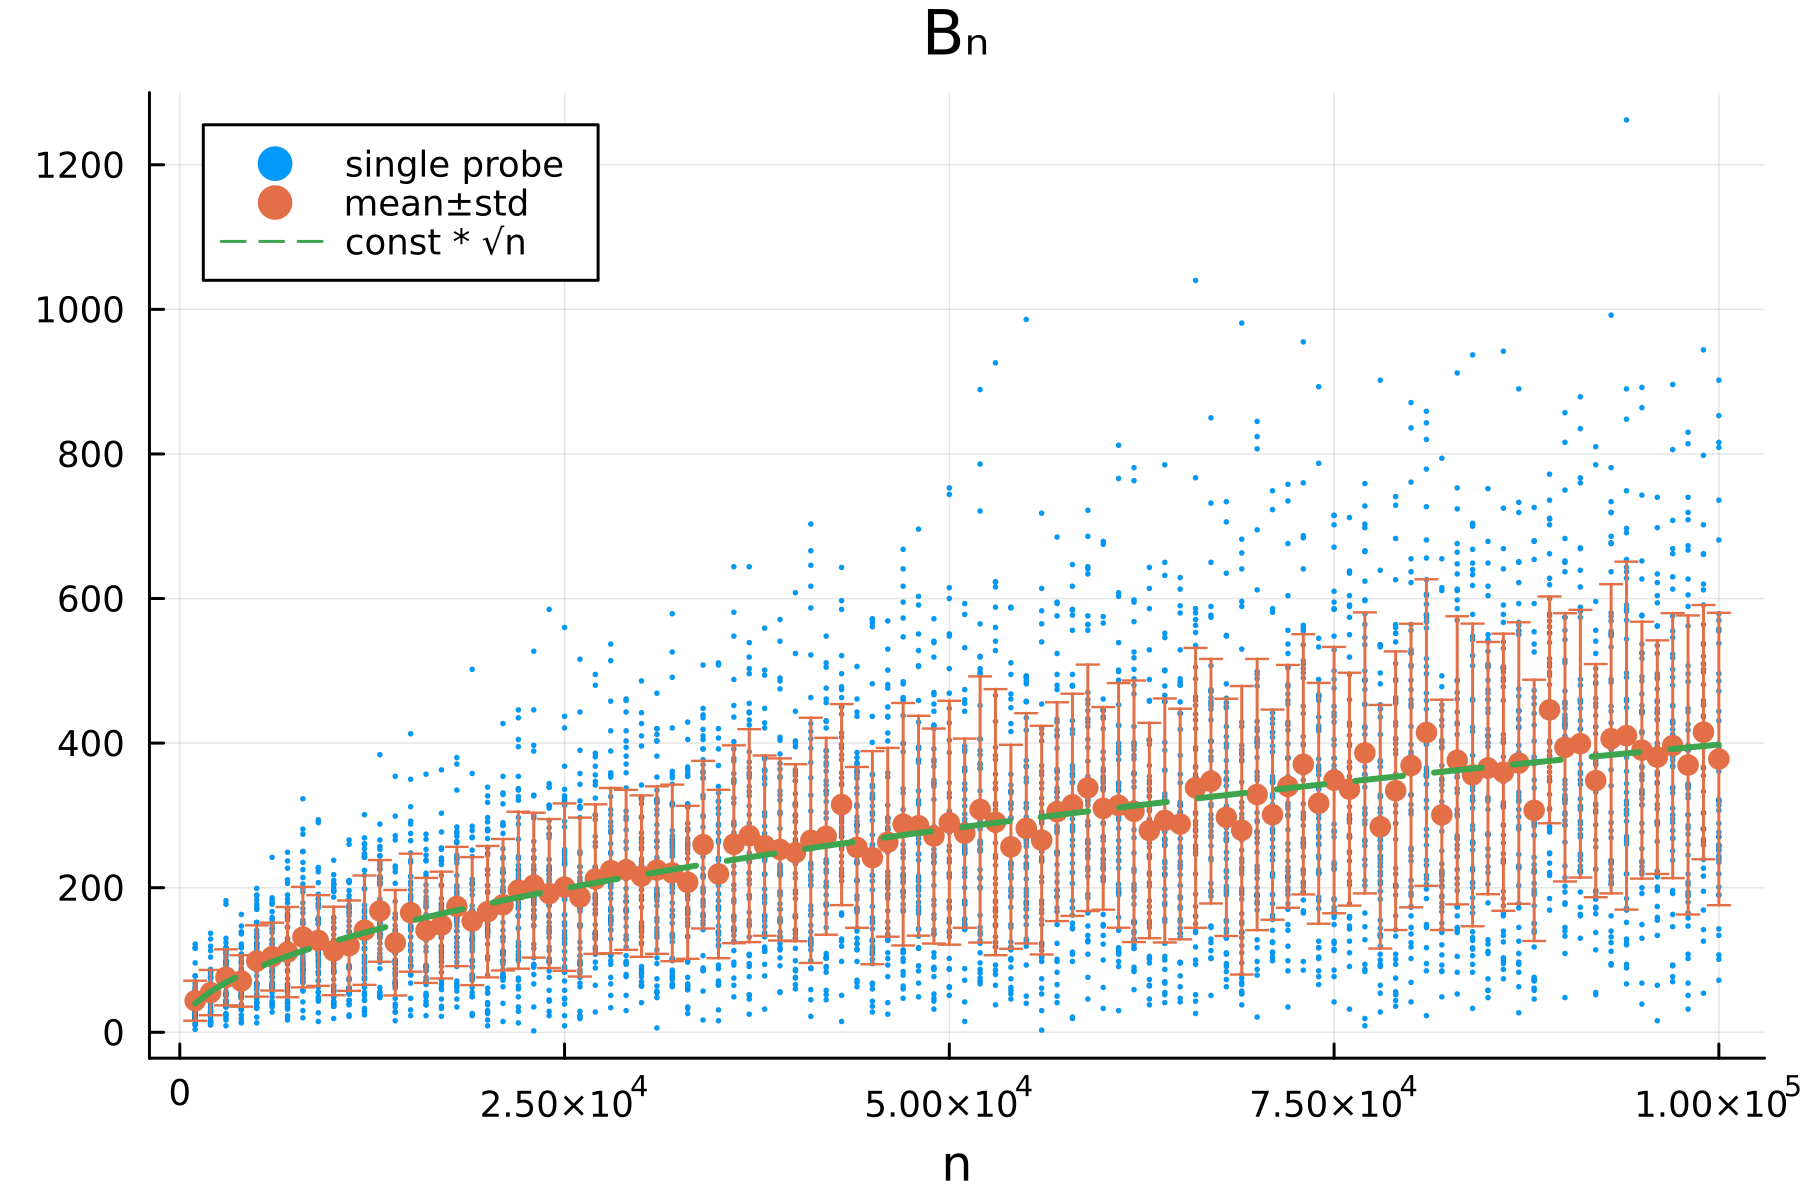
\includegraphics[width=1.0\textwidth]{../results/B_n.png}
    \caption{Moment pierwszej kolizji $B_n$, wraz z zaznaczonymi wartościami średnimi z $k$ powtórzeń, oraz ich odchyleniem standardowym. Przy większej ilości urn ($n$) odchylenie standardowe, czyli rozrzut punktów zwiększa się, a ich średnia wartość rośnie proporcjonalnie do $const \cdot \sqrt{n}$. Stała $const$ została przyjęta jako średnia z wartości $\frac{B_n}{\sqrt{n}}$, nie jest to dokładne dopasowanie funkcji, a jedynie zgrubne pokazanie generalnego trendu.}
    \label{fig:B_n}
\end{figure}

\begin{figure}
    \centering
    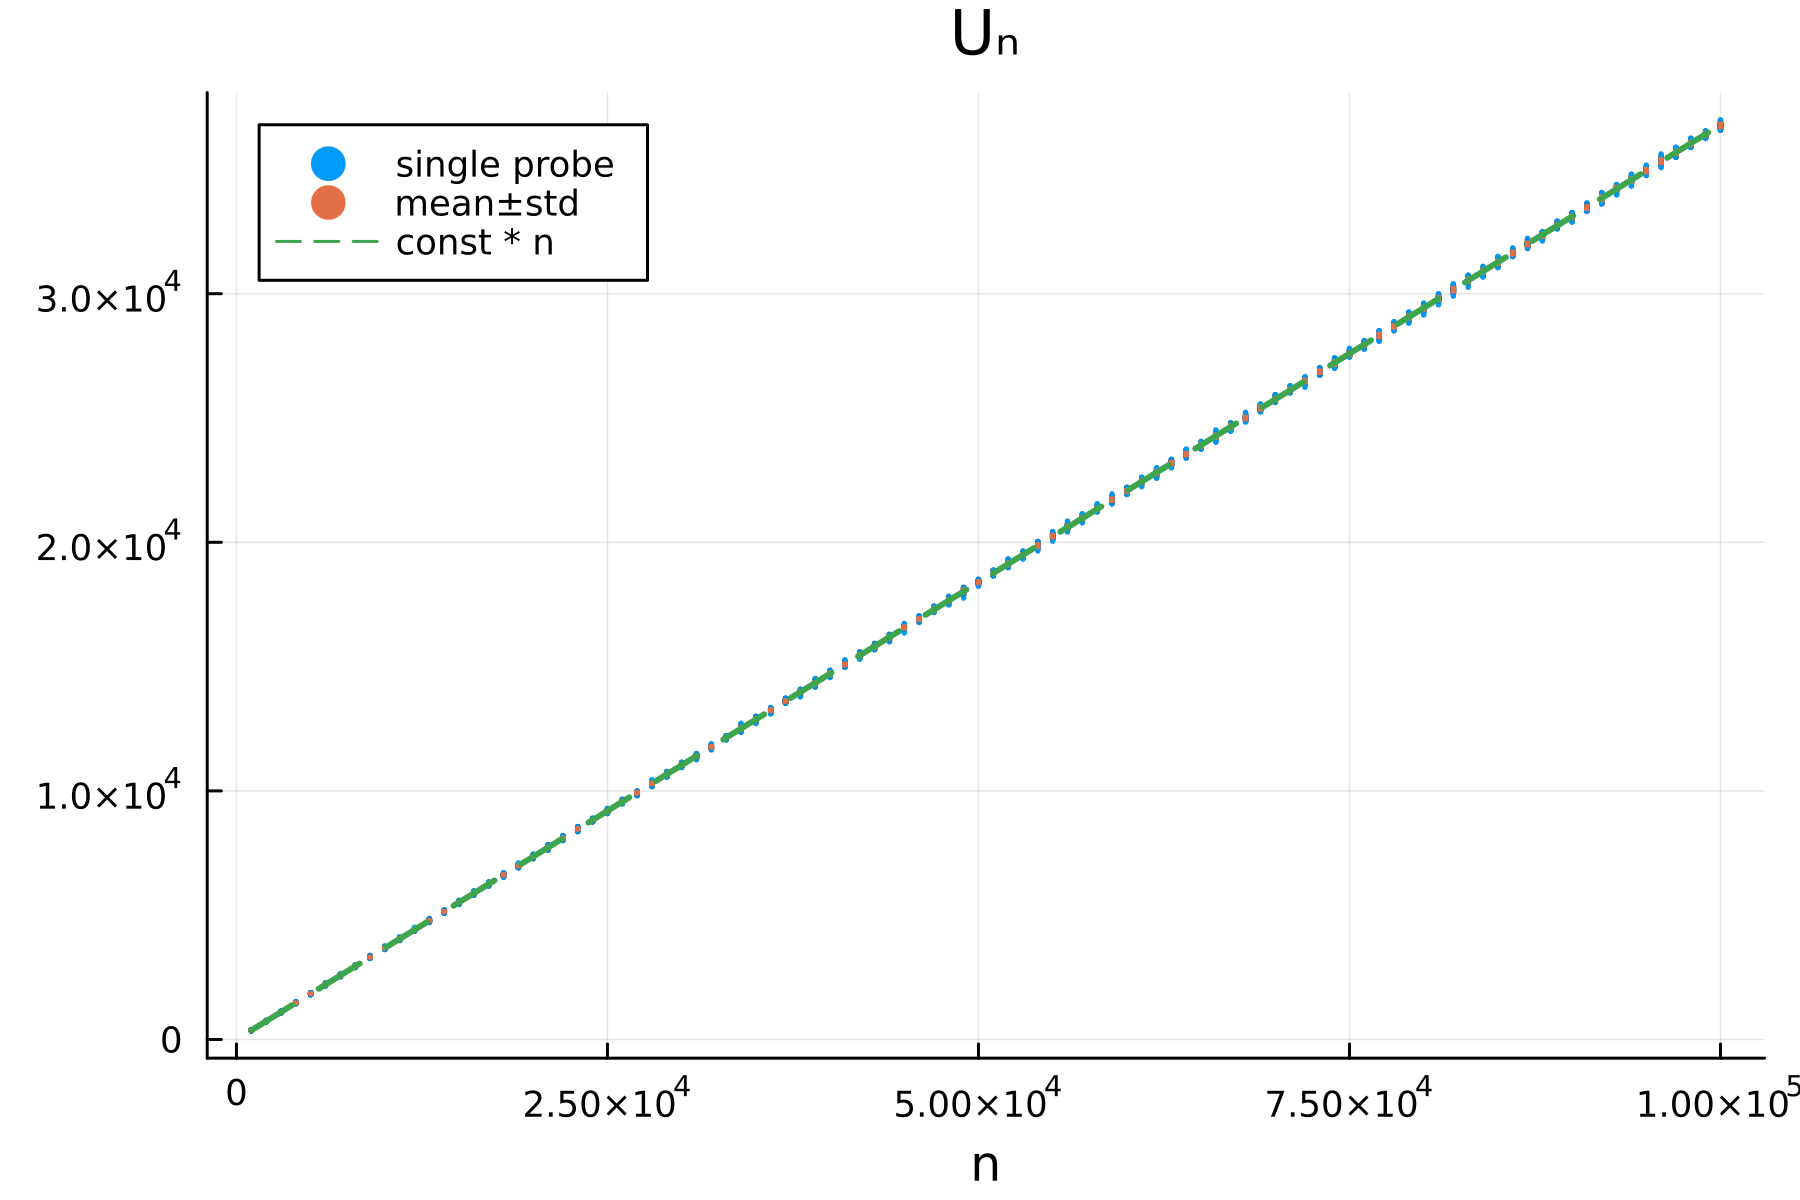
\includegraphics[width=1.0\textwidth]{../results/U_n.png}
    \caption{Liczba pustych urn $U_n$ po wrzuceniu $n$ kul, wraz z zaznaczonymi wartościami średnimi z $k$ powtórzeń, oraz ich odchyleniem standardowym. Punkty są mocno skoncentrowane na prostej, na wykresie prawie nie widać ich rozrzutu, jest on w skali wykresu bardzo mały oraz niezależny od $n$. Wartości $U_n$ rosną proporcjonalnie do $const \cdot n$. Stała $const$ została przyjęta jako średnia z wartości $\frac{U_n}{n}$, nie jest to dokładne dopasowanie funkcji, a jedynie zgrubne pokazanie generalnego trendu.}
    \label{fig:U_n}
\end{figure}

\begin{figure}
    \centering
    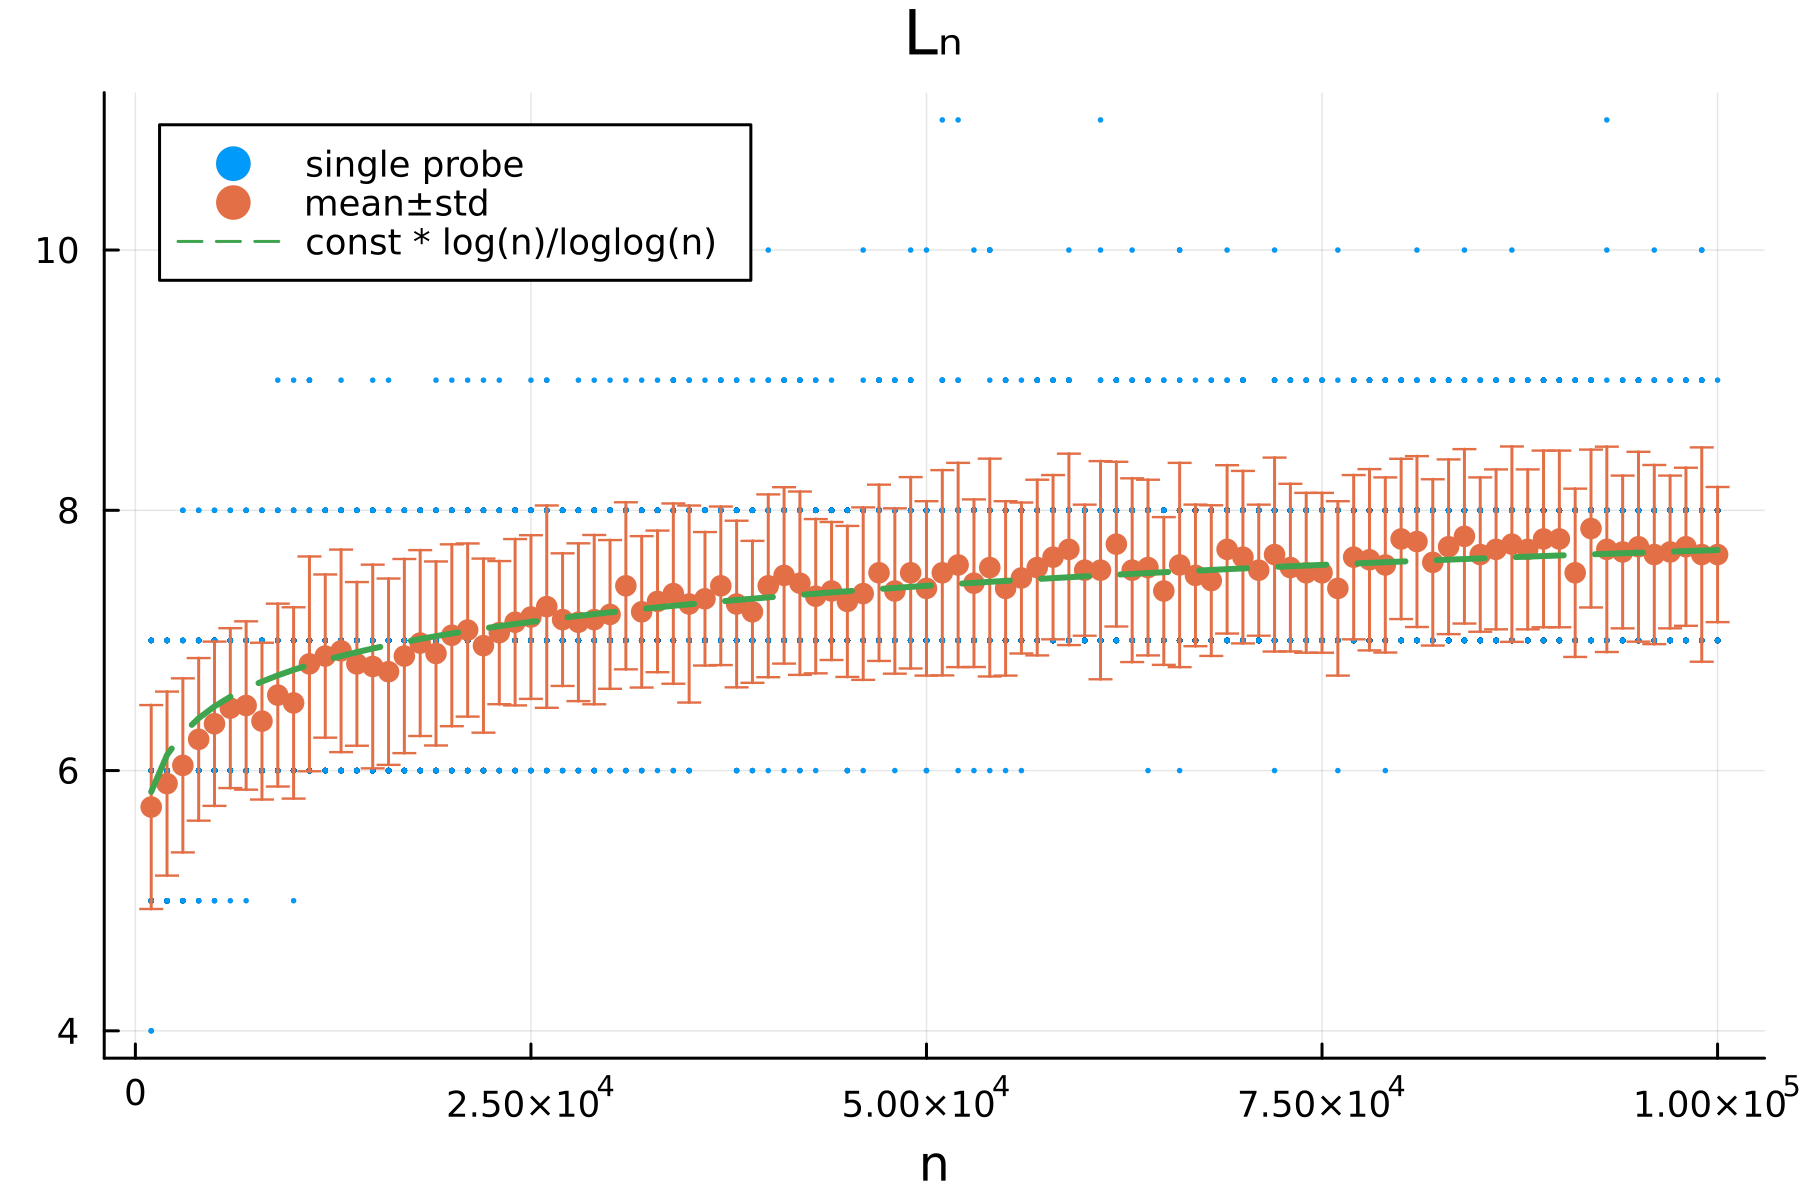
\includegraphics[width=1.0\textwidth]{../results/L_n.png}
    \caption{Maksymalna liczba kul w urnie $L_n$ po wrzuceniu $n$ kul, wraz z zaznaczonymi wartościami średnimi z $k$ powtórzeń, oraz ich odchyleniem standardowym. Odchylenie standardowe wydaje się być niezależnie od $n$.
        Średnie wartości $L_n$ rosną proporcjonalnie do $const \cdot \frac{\ln n}{\ln\ \ln n}$. Stała $const$ została przyjęta jako średnia z wartości $\frac{L_n}{\frac{\ln n}{\ln\ \ln n}}$, nie jest to dokładne dopasowanie funkcji, a jedynie zgrubne pokazanie generalnego trendu.}
    \label{fig:L_n}
\end{figure}

\begin{figure}
    \centering
    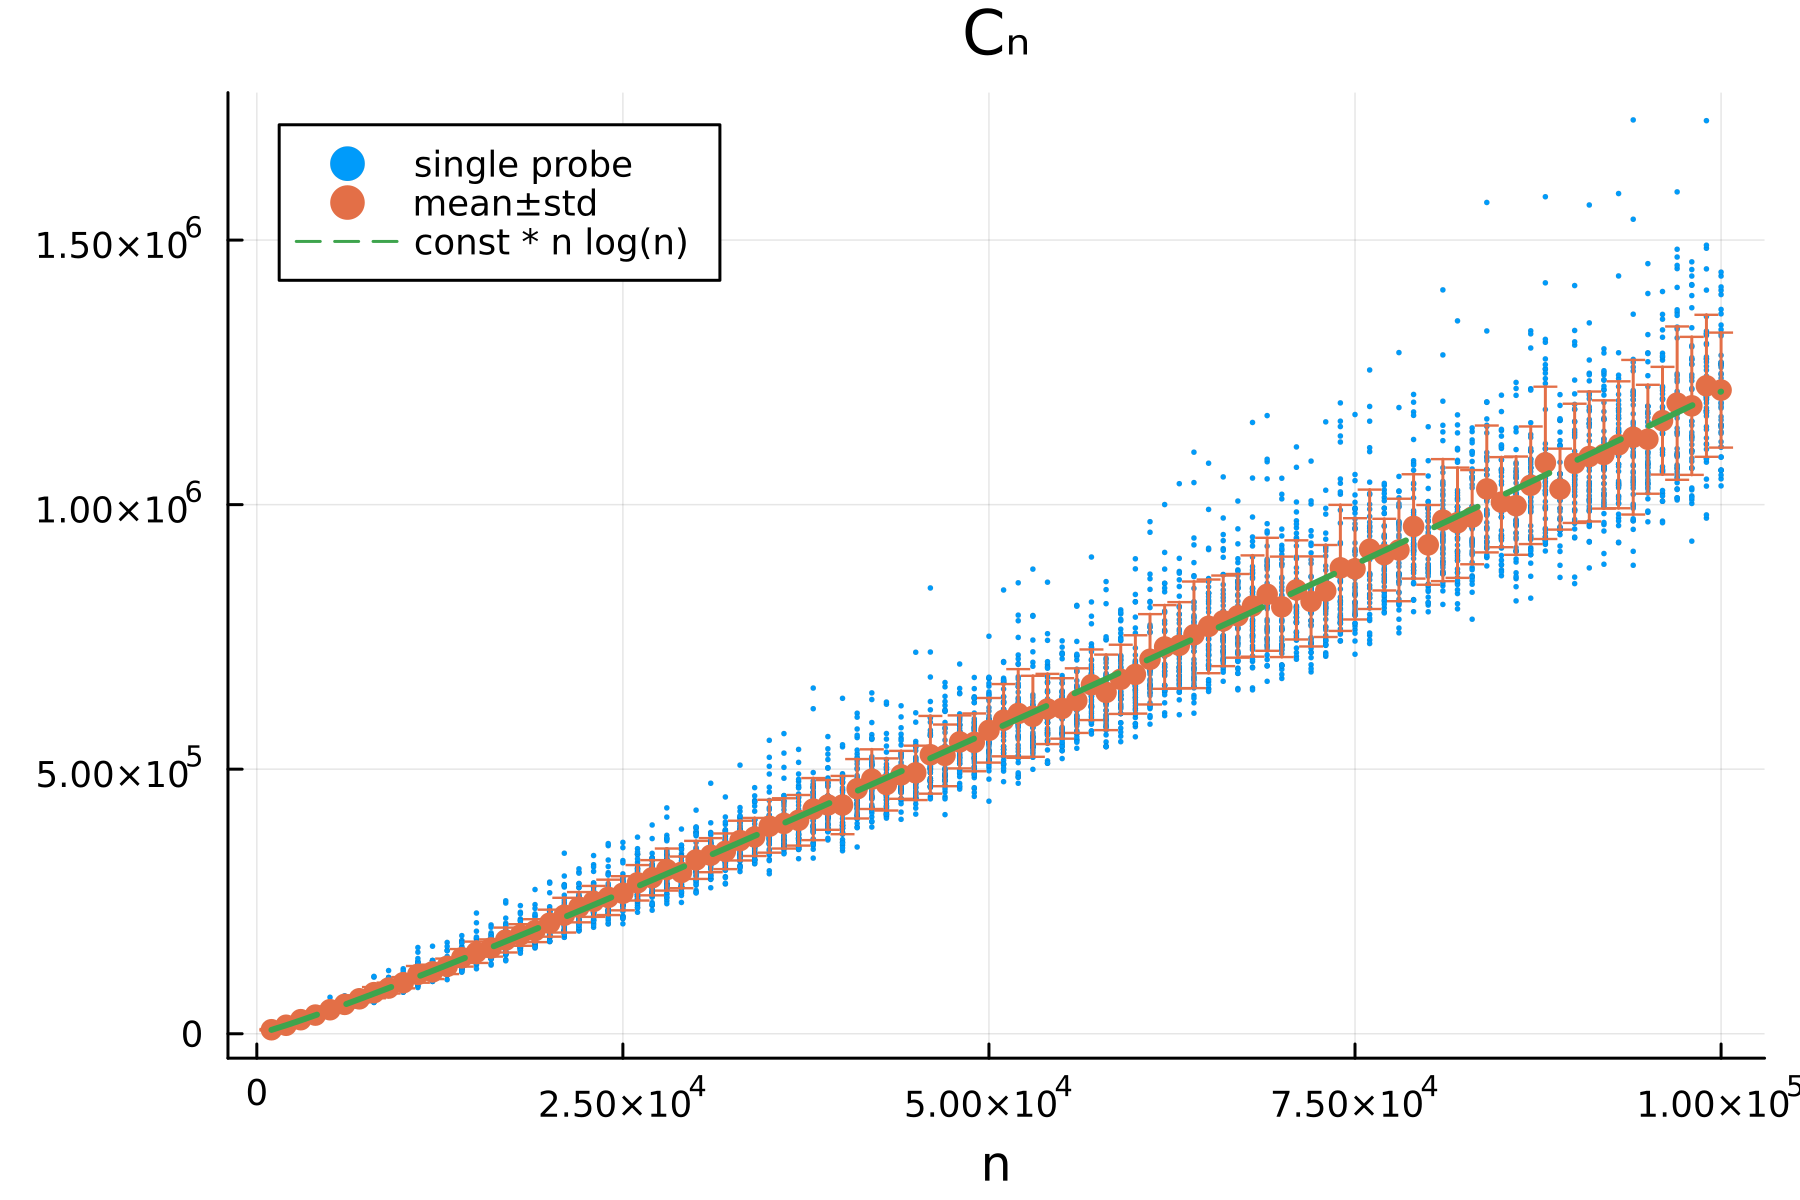
\includegraphics[width=1.0\textwidth]{../results/C_n.png}
    \caption{Minimalna liczba rzutów $C_n$, po której w każdej z urn jest co najmniej jedna kula (\textit{coupon collector's problem}), wraz z zaznaczonymi wartościami średnimi z $k$ powtórzeń, oraz ich odchyleniem standardowym. Odchylenie standardowe (odpowiadające rozrzutowi punktów od średniej) zwiększa się wraz ze wzrostem $n$.
        Wartości $C_n$ rosną proporcjonalnie do $const \cdot n \ln n$. Stała $const$ została przyjęta jako średnia z wartości $\frac{C_n}{n \ln n}$, nie jest to dokładne dopasowanie funkcji, a jedynie zgrubne pokazanie generalnego trendu.}
    \label{fig:C_n}
\end{figure}

\begin{figure}
    \centering
    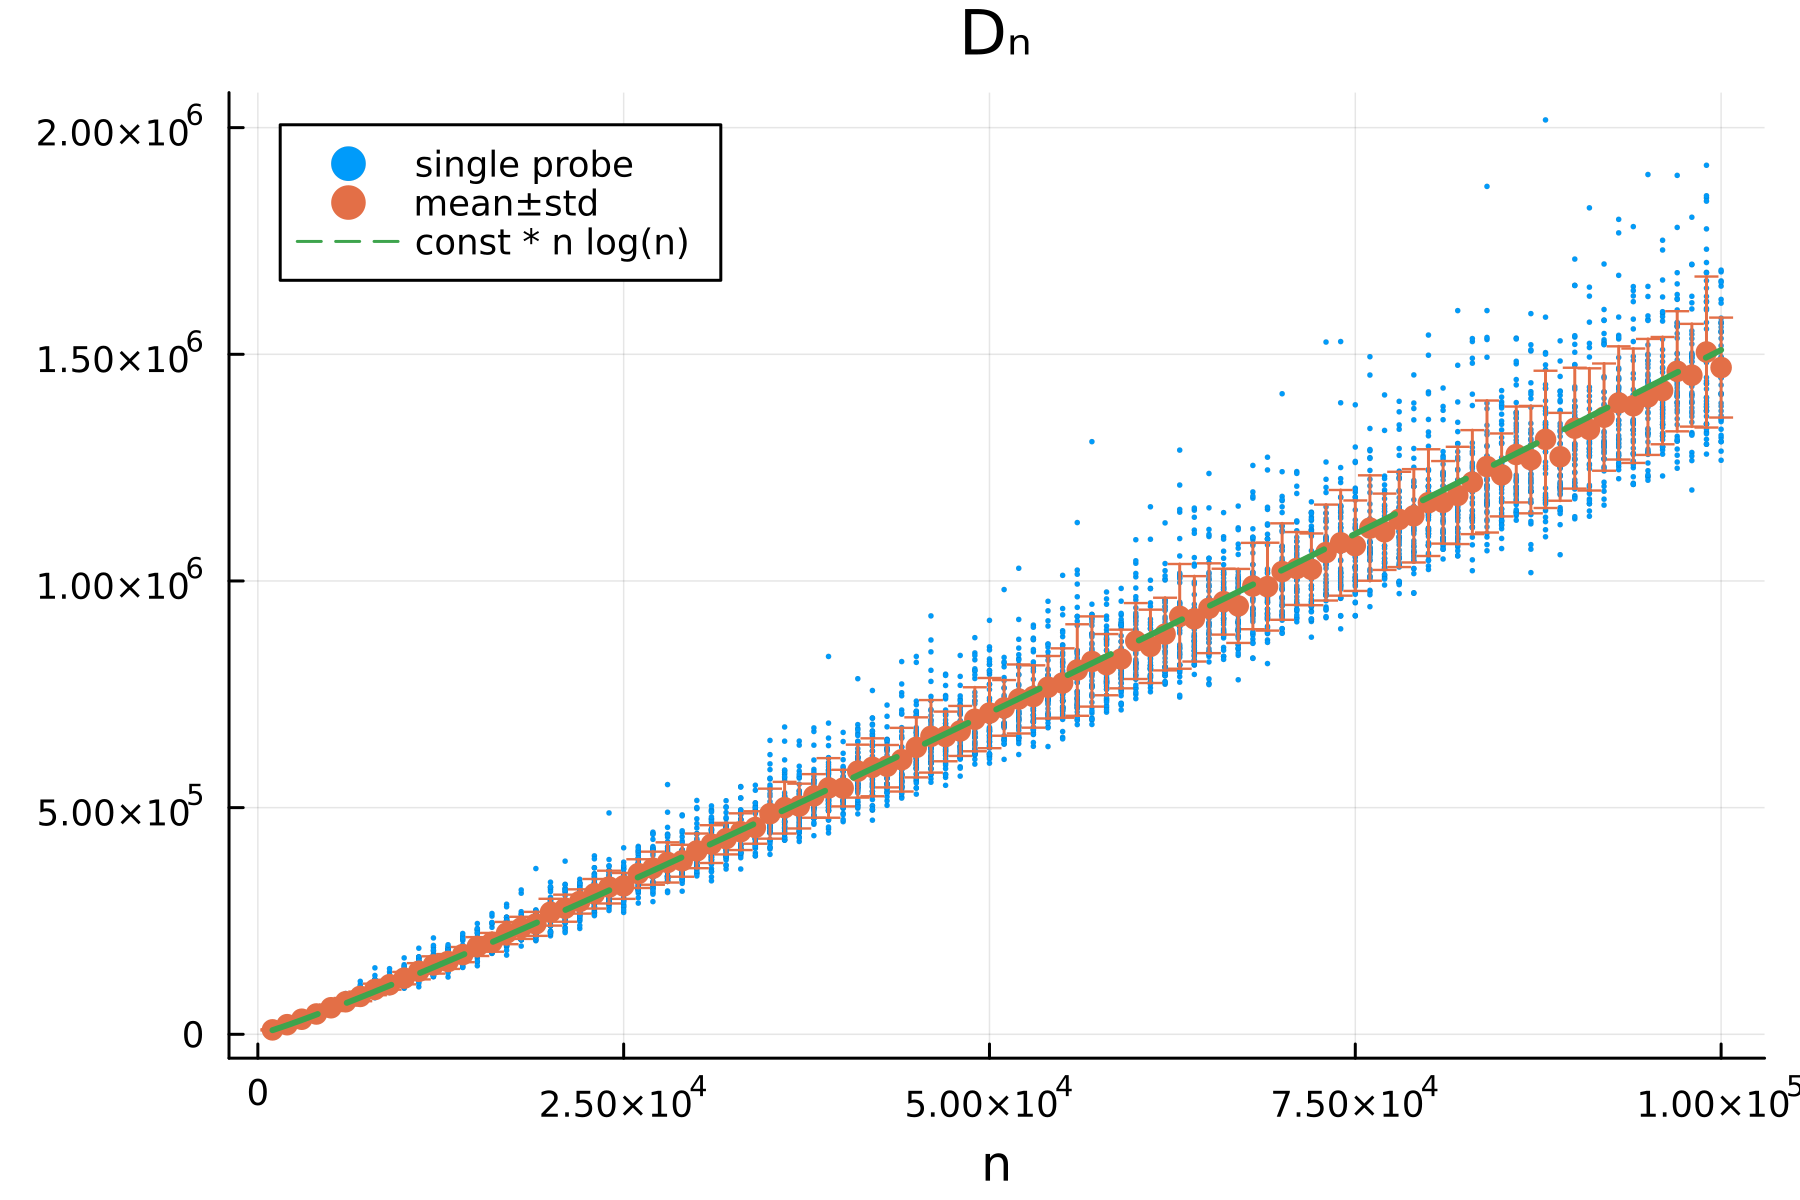
\includegraphics[width=1.0\textwidth]{../results/D_n.png}
    \caption{Minimalna liczba rzutów $D_n$, po której w każdej z urn są co najmniej dwie kule (\textit{siblings of the coupon collector}), wraz z zaznaczonymi wartościami średnimi z $k$ powtórzeń, oraz ich odchyleniem standardowym. Odchylenie standardowe (odpowiadające rozrzutowi punktów od średniej) zwiększa się wraz ze wzrostem $n$.
        Wartości $D_n$ rosną proporcjonalnie do $const \cdot n \ln n$. Stała $const$ została przyjęta jako średnia z wartości $\frac{D_n}{n \ln n}$, nie jest to dokładne dopasowanie funkcji, a jedynie zgrubne pokazanie generalnego trendu.}
    \label{fig:D_n}
\end{figure}

\begin{figure}
    \centering
    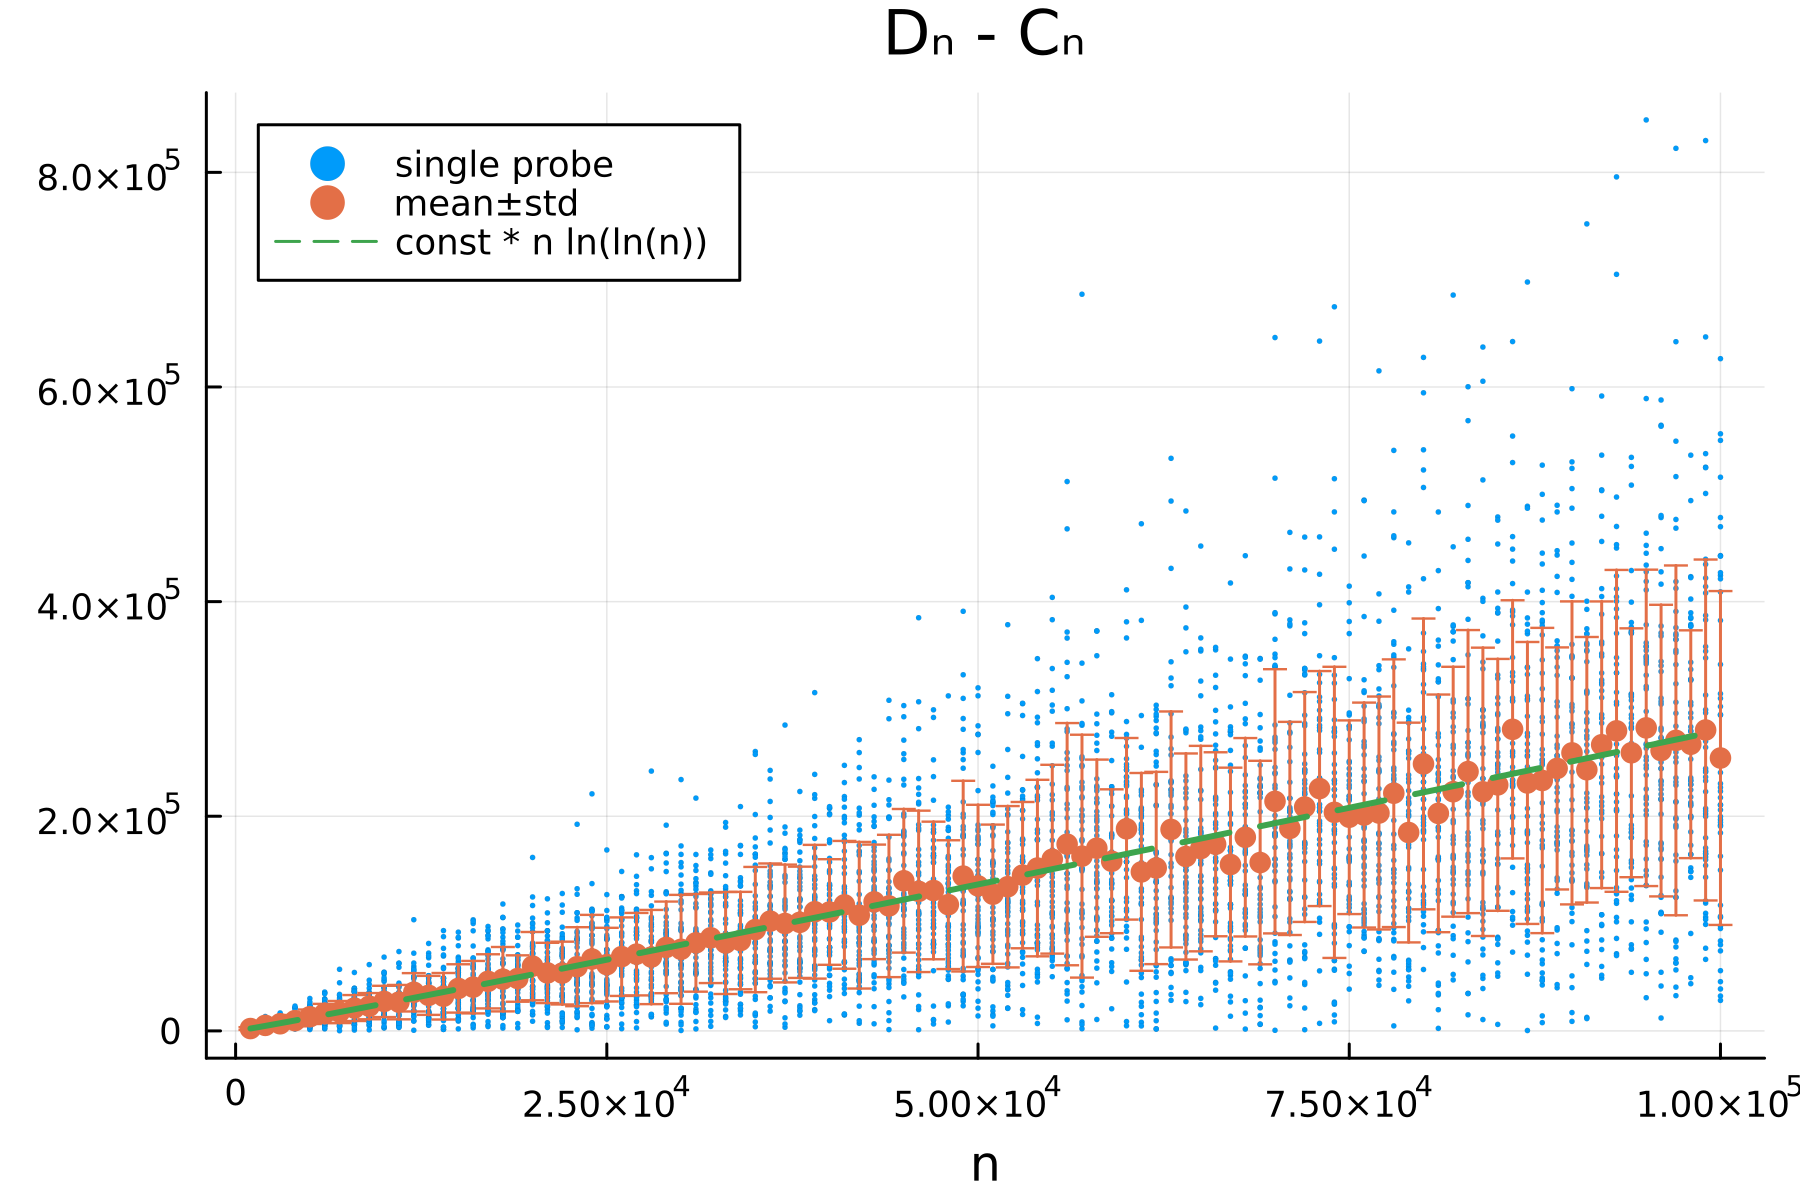
\includegraphics[width=1.0\textwidth]{../results/D_n-C_n.png}
    \caption{Liczba rzutów od momentu $C_n$ (w każdej urnie jest przynajmniej jedna kula) do momentu $D_n$ (w każdej urnie są przynajmniej dwie kule) wraz z icha wartościami średnimi oraz oddchyleniem standardowym. Rozrzut punktów od średniej (odchylenie standardowe) zwiększa się znacząco wraz ze wzrostem liczby urn.  Wartości $D_n - C_n$ rosną proporcjonalnie do $const \cdot n \ln \ln n$. Stała $const$ została przyjęta jako średnia z wartości $\frac{D_n - C_n}{n \ln \ln n}$, nie jest to dokładne dopasowanie funkcji, a jedynie zgrubne pokazanie generalnego trendu.}
    \label{fig:D_n-C_n}
\end{figure}

\section{Pomocnicze wykresy}
$b, u, l, c, d$ oznaczają wartości średnie odpowiednio $B_n, U_n, L_n, C_n, D_n$. Narysowano dla nich wykresy, aby znaleźć funkcję do której są proporcjonalne.

\begin{figure}[h]
    \centering
    \begin{subfigure}[b]{0.49\textwidth}
        \centering
        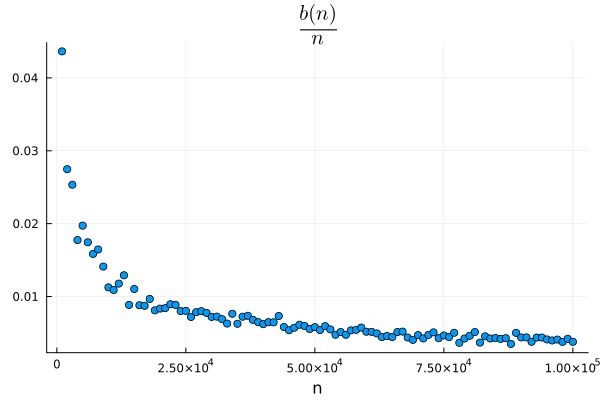
\includegraphics[width=1.0\textwidth]{../results/b(n)_1.png}
        \caption{$/ n$}
    \end{subfigure}
    \begin{subfigure}[b]{0.49\textwidth}
        \centering
        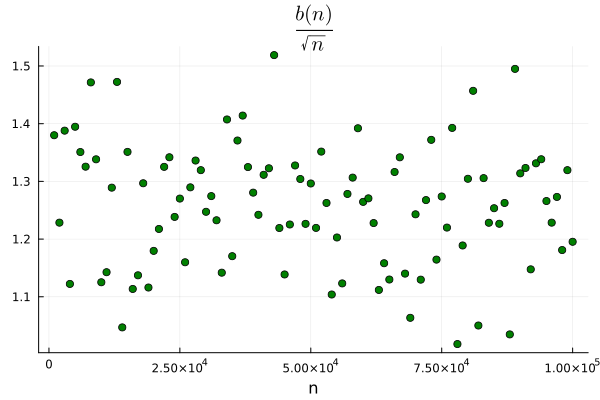
\includegraphics[width=1.0\textwidth]{../results/b(n)_2.png}
        \caption{$/ \sqrt{n}$}
    \end{subfigure}
    \caption{Funkcje średniej wartości $B_n$ od $n$, na zielono zaznaczono funkcję, która najbardziej wydaje się zbiegać do stałej (Rys. b). Dla dużych $n$ średnia wartość $B_n$ jest proporcjonalna do $\sqrt{n}$.}
\end{figure}

\begin{figure}[h]
    \centering
    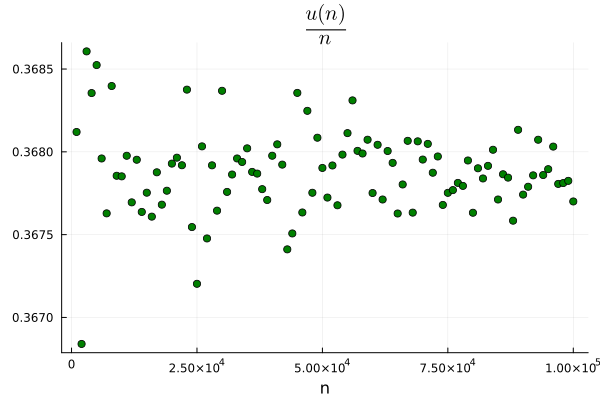
\includegraphics[width=0.5\textwidth]{../results/u(n)_1.png}
    \caption{Funkcja średniej wartości $U_n$ od $n$, wydaje się ona zbiegać do stałej, więc średnia wartość $U_n$ zależy liniowo od $n$. }
\end{figure}

\begin{figure}[h]
    \centering
    \begin{subfigure}{0.32\textwidth}
        \centering
        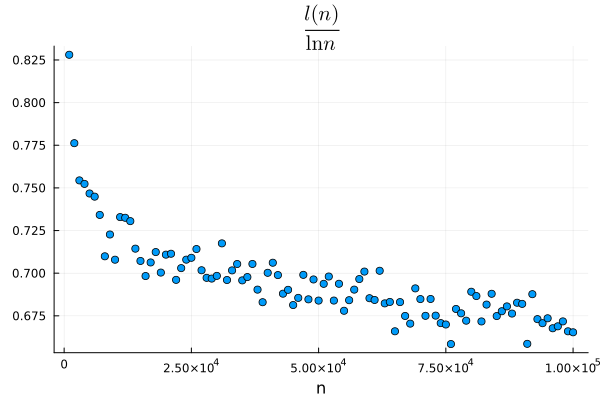
\includegraphics[width=1.0\textwidth]{../results/l(n)_1.png}
        \caption{$/\ln n$}
    \end{subfigure}
    \begin{subfigure}{0.32\textwidth}
        \centering
        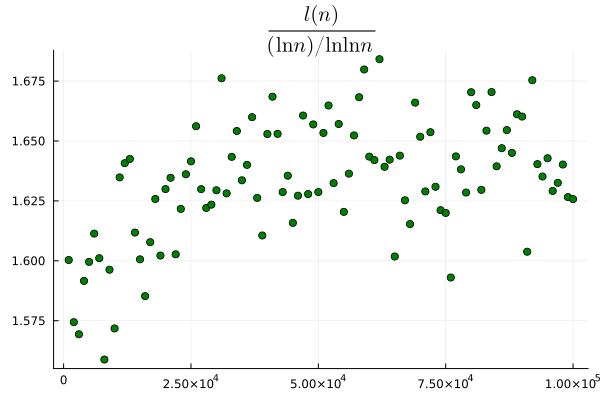
\includegraphics[width=1.0\textwidth]{../results/l(n)_2.png}
        \caption{$/\frac{\ln n}{\ln \ln n}$}
    \end{subfigure}
    \begin{subfigure}{0.32\textwidth}
        \centering
        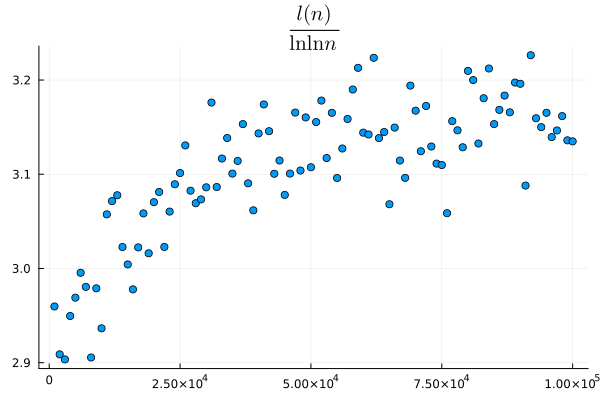
\includegraphics[width=1.0\textwidth]{../results/l(n)_3.png}
        \caption{$/ \ln\ln n$}
    \end{subfigure}
    \caption{Funkcje średniej wartości $L_n$ od $n$. Na zielono zaznaczono funkcję która wydaje się zbiegać do stałej (Rys. b). Dla dużych $n$ średnia wartość $L_n$ jest proporcjonalna do $\frac{\ln n}{\ln \ln n}$.}
\end{figure}

\begin{figure}[h]
    \centering
    \begin{subfigure}{0.32\textwidth}
        \centering
        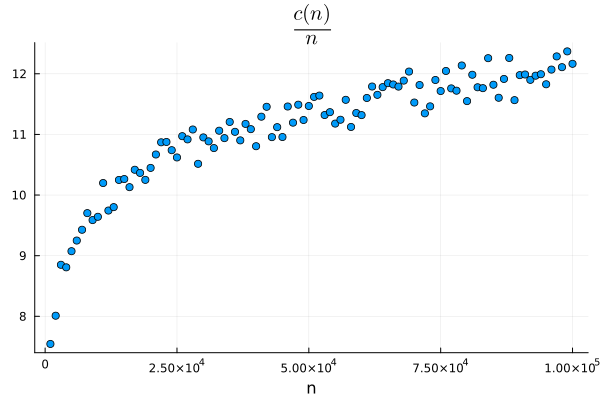
\includegraphics[width=1.0\textwidth]{../results/c(n)_1.png}
        \caption{$/ n$}
    \end{subfigure}
    \begin{subfigure}{0.32\textwidth}
        \centering
        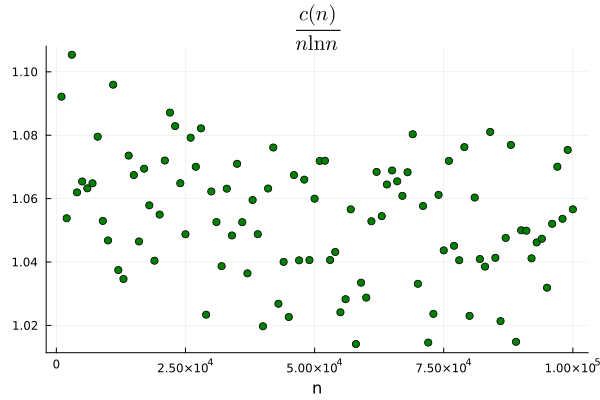
\includegraphics[width=1.0\textwidth]{../results/c(n)_2.png}
        \caption{$/ n \ln n$}
    \end{subfigure}
    \begin{subfigure}{0.32\textwidth}
        \centering
        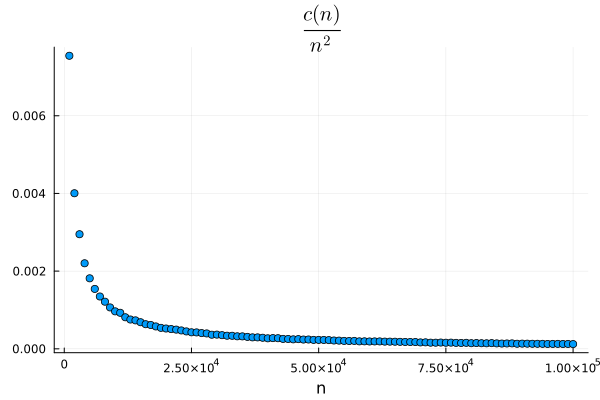
\includegraphics[width=1.0\textwidth]{../results/c(n)_3.png}
        \caption{$/ n^2$}
    \end{subfigure}
    \caption{Funkcje średniej wartości $C_n$ od $n$. Na zielono zaznaczono funkcję która wydaje się zbiegać do stałej (Rys. b). Dla dużych $n$ średnia wartość $C_n$ jest proporcjonalna do $n\ln n$.}
\end{figure}

\begin{figure}[h]
    \centering
    \begin{subfigure}{0.32\textwidth}
        \centering
        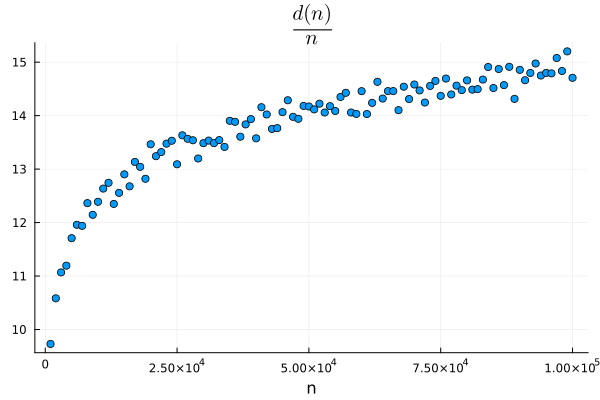
\includegraphics[width=1.0\textwidth]{../results/d(n)_1.png}
        \caption{$/ n$}
    \end{subfigure}
    \begin{subfigure}{0.32\textwidth}
        \centering
        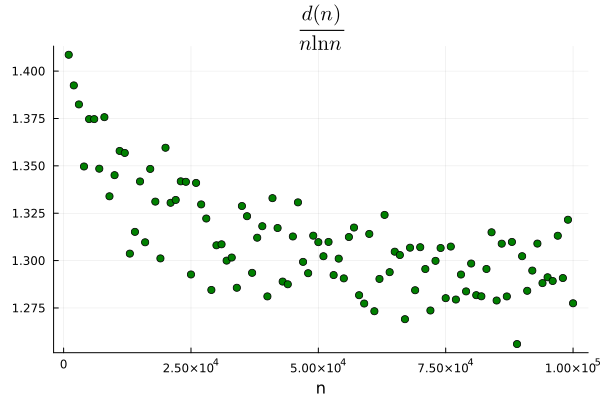
\includegraphics[width=1.0\textwidth]{../results/d(n)_2.png}
        \caption{$/ n \ln n$}
    \end{subfigure}
    \begin{subfigure}{0.32\textwidth}
        \centering
        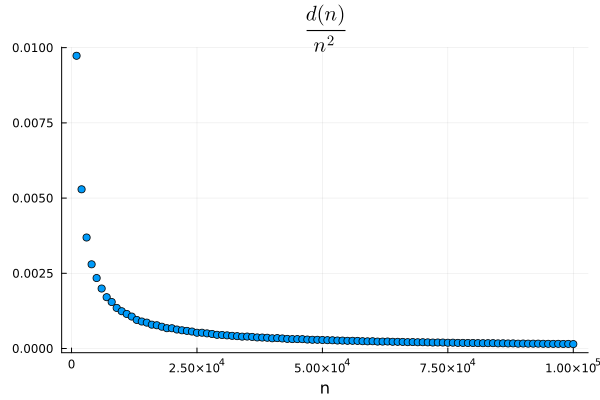
\includegraphics[width=1.0\textwidth]{../results/d(n)_3.png}
        \caption{$/ n^2$}
    \end{subfigure}
    \caption{Funkcje średniej wartości $D_n$ od $n$. Na zielono zaznaczono funkcję która wydaje się zbiegać do stałej (Rys. b). Dla dużych $n$ średnia wartość $D_n$ jest proporcjonalna do $n\ln n$.}
\end{figure}

\begin{figure}[h]
    \centering
    \begin{subfigure}{0.32\textwidth}
        \centering
        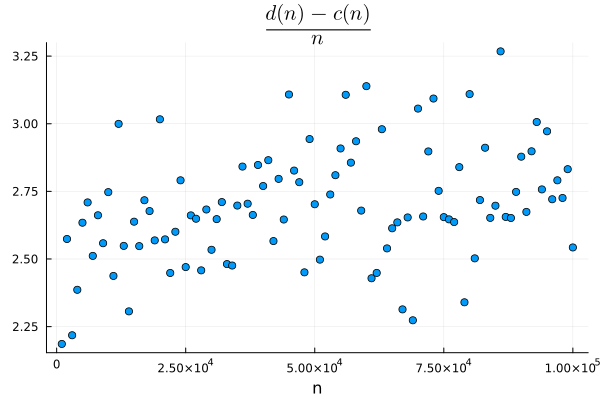
\includegraphics[width=1.0\textwidth]{../results/d(n)-c(n)_1.png}
        \caption{$/ n$}
    \end{subfigure}
    \begin{subfigure}{0.32\textwidth}
        \centering
        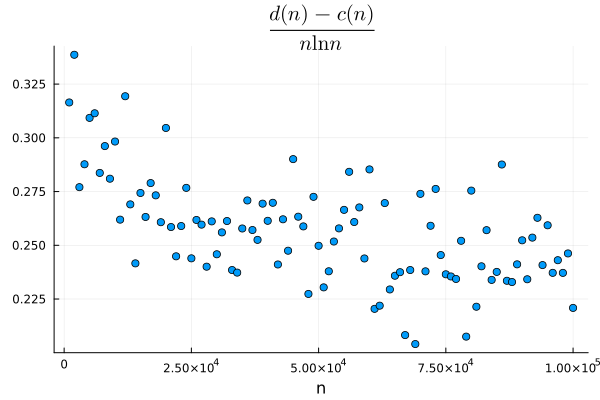
\includegraphics[width=1.0\textwidth]{../results/d(n)-c(n)_2.png}
        \caption{$/ n \ln n$}
    \end{subfigure}
    \begin{subfigure}{0.32\textwidth}
        \centering
        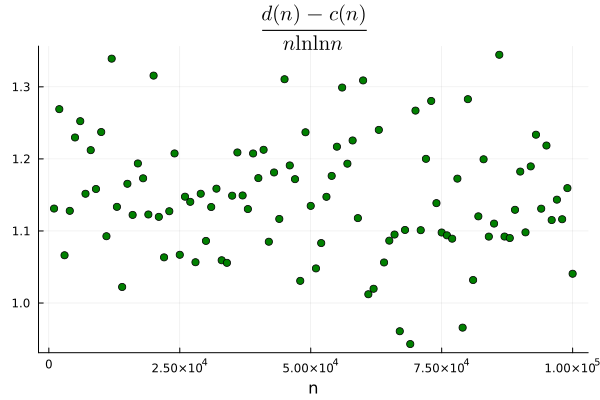
\includegraphics[width=1.0\textwidth]{../results/d(n)-c(n)_3.png}
        \caption{$/ n \ln \ln n$}
    \end{subfigure}
    \caption{Funkcje średniej wartości $D_n-C_n$ od $n$. Na zielono zaznaczono funkcję która wydaje się zbiegać do stałej (Rys. c). Dla dużych $n$ średnia wartość $C_n$ jest proporcjonalna do $n\ln\ln n$.}
\end{figure}


\section{Wnioski}
Do znajdywania asymptotyki wartości średnich korzystano z własności
$$
    x \sim f(n) \iff \frac{x}{f(n)} \sim const
$$
Nie była to jednak do końca prawdziwa zależność, tylko jej przybliżenie, ponieważ w $f(n)$ uwzględniano tylko najbardziej liczący się człon, a pomijano te mniej znaczące. Jest jednak ono wystarczające na potrzeby tego eksperymentu.

Z pomocniczych wykresów wynika, że wartości średnie są zależne od $n$ jak:
\begin{itemize}
    \item $b(n) \sim \sqrt{n}$
    \item $u(n) \sim n$
    \item $l(n) \sim \frac{\ln n}{\ln \ln n}$
    \item $c(n) \sim n\ln n$
    \item $d(n) \sim n\ln n$
    \item $d(n)-c(n) \sim n\ln \ln n$
\end{itemize}

Minimalna liczba rzutów, po której w każdej z urn jest co najmniej jedna kula ($C_n$)stanowi analogię do \textit{coupon collector's problem} - problemu kolekcjonera kuponów. W tym przypadku liczba różnych kuponów jest równa liczbie urn ($n$), a minimalna liczba rzutów $C_n$ jest równa liczbie kuponów, które musi kolekcjoner zebrać, aby mieć jeden kupon każdego rodzaju. W problemie tym zakładamy, że każdy rodzaj kuponu ma takie samo prawdopodobieństwo wystąpienia, jak samo jak każda urna ma takie samo prawdopodobieństwo, że wpadnie do niej losowana kula. Liczba $D_n$ natomiast odpowiada problemowi brata kolekcjonera kuponów (\textit{coupon collector's brother}), w którym kolekcjoner musi zebrać wszystkie kupony dla siebie, oraz swojego brata, czyli efektywnie musi mieć po 2 kupony każdego rodzaju. W jeszcze ogólniejszej wersji tego problemu - \textit{the siblings of the coupon collector} kolekcjoner musi zebrać po $k$ kuponów każdego rodzaju, gdzie $k$ jest liczbą jego rodzeństwa, to uogólnienie nie było jednak rozważane w tym eksperymencie.

Liczba pierwszej kolizji, czyli moment w krótym pierwszy raz kula wpadła do niepustej urny nazywa się \textit{birthday paradox}, z uwagi na podobieństwo do paradoksu urodzinowego, zgodnie z którym w grupie 23 osób prawdopodobieństwo, że dwie osoby urodziły się tego samego dnia wynosi 50\%. Liczba urn $n$ jest analogiczna do liczby dni ($n=365$ w paradoksie urodzinowym), a $B_{365}$ jest analogiczne do liczby osób które spotykamy, dopóki dwie z tych osób nie urodziły się tego samego dnia w roku.

\textit{Birthday paradox} w kontekście funkcji hashujących jest powiązany z częstością występowania kolizji w tych funkcjach. Jeśli $n$ będzie liczbą wszystkich możliwych kombinacji hashy, które na wyjściu może wygenerować funkcja, to $B_n$ nam powie ile przedmiotów możemy dodawać do zbioru, aż do momentu gdy dwa z nich dostaną ten sam hash (z zastrzeżeniem, że w eksperymencie \textit{balls and bins} każda kula była wrzucana niezależnie od innych, a urny były losowane z rozkładu jednorodnego, co nie zawsze jest spełnione w fukcjach hashujących, szczególnie tych niekryptograficznych - nie każdy hash ma taką samą "szansę" na bycie trafionym, oraz "odległość" między kluczami może mieć wpływ na wyjściowy hash). Stwarza to np problem w słownikach (\textit{hashmap}), gdzie jeśli dodamy zbyt wiele elementów i wystąpi kolizja, to stracimy dane. Wybiera się więc takie funkcje hashujące, które zwracają odpowiednio dużą ilość możliwych hashy, aby kolizja nie nastąpiła w praktycznych zastosowaniach, mając też na uwadze szybkość działania funkcji.

Kryptograficzne funkcje hashujące to taka podgrupa funkcji hashujących, w których mniej liczy się szybkość wykonywania funkcji, a bardziej jej niezawodność i odporność na ataki. Czyli dopuszczalny moment pierwszej kolizji ($B_n$) będzie dużo późniejszy (oczekiwane $B_n$ będzie dużo większe). Kryptograficzne funkcje hashujące powinny też być odporne na ataki, w których ktoś będzie chciał doprowadzić do kolizji, więc np. "podobieństwo" elementów wejściowych nie powinno mieć znaczenia, tak jak przy losowaniu urny nie mają znaczenia kule wrzucone wcześniej, ponieważ każde zdarzenie jest niezależne od poprzednich.

% Kryptograficzne funkcje hashujące, są wykorzystywane m.in. do podpisywania programów, aby mieć pewność, że użytkownik instaluje niezmodyfikowany program od źródła. Jeśli moment pierwszej kolizji następowałby zbyt szybko, to ktoś mógłby pobrać program, zmodyfikować go (np. podpinając wirusa) i stworzyć $B_n$ kopii tego programu, praktycznie identycznych, różniących się tylko nieznacznymi szczegółami, aż któraś z nich miała by identyczny podpis co oryginał. Użytkownik mógłby wtedy pobrać program, który wyglądałby na oryginał, ale byłby zainfekowany wirusem.


Eksperyment wykonano w języku Julia 1.7.2, jako generator liczb losowych wykorzystano Xoshiro256++ - domyślnego generatora języka Julia.

\end{document}
